% Set up the document
\documentclass{article}

% Page size
\usepackage[
    letterpaper,]{geometry}

% Lines between paragraphs
\setlength{\parskip}{\baselineskip}
\setlength{\parindent}{0pt}

% Math
\usepackage{mathtools}
\usepackage{amssymb}
\usepackage{commath}

% Math notation macros
\newcommand{\R}{\mathbb{R}}
\newcommand{\Z}{\mathbb{Z}}

\def\*#1{\mathbf{#1}}
\def\ti#1{\tilde{#1}}
\newcommand{\dadvd}[2]{\dfrac{\text{D} #1}{\text{D} #2}} % advective derivative

\newcommand{\fS}{\mathcal{S}} % fancy S
\newcommand{\tphi}{\tilde{\phi}}
\newcommand{\nhat}{\mathbf{\hat{n}}}
\newcommand{\rhat}{\mathbf{\hat{r}}}
\newcommand{\thetahat}{\boldsymbol{\hat{\theta}}}
\newcommand{\xhat}{\mathbf{\hat{x}}}
\newcommand{\yhat}{\mathbf{\hat{y}}}
\newcommand{\zhat}{\mathbf{\hat{z}}}
\newcommand{\omegavec}{\boldsymbol{\omega}}
\newcommand{\tauvec}{\boldsymbol{\tau}}

% Links
\usepackage{hyperref}

% Page numbers at top right
\usepackage{fancyhdr}
\pagestyle{fancy}
\fancyhf{}
\fancyhead[R]{\thepage}
\renewcommand\headrulewidth{0pt}

% Graphics
\usepackage{float}
\usepackage{graphicx}
\graphicspath{ {./img/} }

\begin{document}

\textbf{MATH 462 Assignment 11} \\
\textbf{Matt Wiens \#301294492} \\
\textbf{2020-04-11}

\textbf{103) Pipe flow.} (3 pages)
Review the notes from 3D Poiseuille pipe flow. The other exact solution
for this case is for flow in a pipe with an annulus cross-section, $S
\leq r \leq R$. The integration in $r$ now allows for keeping the singular term
at $r = 0$.

In addition to solving for the velocity $W(r)$, calculate the mass flux
and the global force balance. Be clear about all the signs in your shear
stress calculation---the cancellation you need is obvious, but the
understanding is in the proper tracing of the signs. Your presentation
of the stress terms will be paid special attention.

\newpage

\textbf{Solution}

Just as in the lecture notes, we will assume the flow is steady and
axisymmetric. Using the incompressible Navier-Stokes equations, we
deduced in lecture that pressure is a function of $z$ only and that the
$z$-velocity $W$ is a function of $r$ only, such that
%
\begin{equation*}
    p_z = - \frac{\Delta p}{L}
    ,
\end{equation*}
%
where $L$ is the length of the pipe, and that
%
\begin{equation}
    \frac{1}{r} \del{r W^\prime(r)}^\prime = - \frac{\Delta p}{\mu L}
    \label{eq:1-1}
    ,
\end{equation}
%
where the prime symbols denote $r$ derivatives. By integrating~\eqref{eq:1-1}
twice, and in doing so being clever to multiply by $r$ before the
first integration and divide by $r$ before the second integration, we
find that the general solution for $W$ is given by
%
\begin{equation*}
    W(r) = - \frac{\Delta p}{4 \mu L} r^2 + c_1 \log r + c_2
    ,
\end{equation*}
%
where $c_1$ and $c_2$ are constants that we need to determine.

To determine the constants $c_1$ and $c_2$ we will invoke ``no-slip''
boundary conditions at the walls of the pipe, so that $W(\pm S) = W(\pm
R) = 0$. These conditions give us that
%
\begin{equation*}
    - \frac{\Delta p}{4 \mu L} S^2 + c_1 \log S + c_2
    = - \frac{\Delta p}{4 \mu L} R^2 + c_1 \log R + c_2
    = 0
    .
\end{equation*}
%
This is a system of two equations in two unknowns which we can solve to
obtain (I used Maple here)
%
\begin{align*}
    c_1 &= \frac{\Delta p}{4 \mu L} \frac{R^2 - S^2}{\log\del{\frac{R}{S}}}, \\
    c_2 &= \frac{\Delta p}{4 \mu L} \frac{S^2 \log R - R^2 \log S}{\log\del{\frac{R}{S}}}
    .
\end{align*}
%
Hence, we can write the velocity $W$ as
%
\begin{align*}
    W(r) &= - \frac{\Delta p}{4 \mu L} r^2
        + \del{\frac{\Delta p}{4 \mu L} \frac{R^2 - S^2}{\log\del{\frac{R}{S}}}} \log r
        + \del{\frac{\Delta p}{4 \mu L} \frac{S^2 \log R - R^2 \log S}{\log\del{\frac{R}{S}}}} \\
         &= \frac{\Delta p}{4 \mu L} \del{S^2 - r^2 + \frac{(R^2 - S^2) \log\del{\frac{r}{S}}}{\log\del{\frac{R}{S}}}}
    .
\end{align*}
%
The simplification obtained in the second line of the above equation can
be obtained by adding zero in the form of
%
\begin{equation*}
    \frac{S^2 \log{S}}{\log\del{\frac{R}{S}}}
    - \frac{S^2 \log{S}}{\log\del{\frac{R}{S}}}
\end{equation*}
%
to the first line of the equation, and then the remaining steps in the
simplification are trivial.

Having determined an explicit formula for $W$, we can now calculate the
mass flux through the pipe with
%
\begin{align*}
    \text{mass flux}
        &= \rho_0 2 \pi \int_S^R W(r) r \dif r \\
        &= \frac{\pi \rho_0 \Delta p}{2 \mu L}
            \int_S^R
                \del{r S^2 - r^3 + r \frac{(R^2 - S^2) \log\del{\frac{r}{S}}}{\log\del{\frac{R}{S}}}}
            \dif r
        .
\end{align*}
%
There is quite a lot to evaluate in the integrand of the above equation,
so we'll do each term separately. For the first term we have
%
\begin{equation*}
    S^2  \int_S^R r \dif r = \frac{S^2 (R^2 - S^2)}{2}
    ;
\end{equation*}
%
for the second term,
%
\begin{equation*}
    \int_S^R r^3 \dif r = \frac{R^4 - S^4}{4}
    ;
\end{equation*}
%
and for the third term,
%
\begin{align*}
    \frac{R^2 - S^2}{\log\del{\frac{R}{S}}}
    \int_S^R r \log\del{\frac{r}{S}} \dif r
    &=
    \frac{R^2 - S^2}{\log\del{\frac{R}{S}}}
    \del{\frac{R^2}{4} \del{2 \log\del{\frac{R}{S}} - 1} + \frac{S^2}{4}}
    \\
    &= \frac{R^2 (R^2 - S^2)}{2} - \frac{(R^2 - S^2)^2}{\log\del{\frac{R}{S}}}
    .
\end{align*}
%
Hence, combining our results, we have
%
\begin{align*}
    \text{mass flux}
        &= \frac{\pi \rho_0 \Delta p}{2 \mu L}
            \del{
                \frac{S^2 (R^2 - S^2)}{2}
                - \frac{R^4 - S^4}{4}
                + \frac{R^2 (R^2 - S^2)}{2}
                - \frac{(R^2 - S^2)^2}{\log\del{\frac{R}{S}}}
            } \\
        &= \frac{\pi \rho_0 \Delta p}{8 \mu L}
            \del{
                R^4 - S^4
                - \frac{(R^2 - S^2)^2}{\log\del{\frac{R}{S}}}
            }
      .
\end{align*}
%
Moving forward to the shear stress, we need there to be a net zero force
in the $z$ direction at $r = S$ and $r = R$ and hence a shear stress to
balance the pressure force. Because the pressure force is in the
positive $z$ direction, the shear force should be in the negative $z$
direction. Calculating the general formula for the shear stress, we have
%
\begin{align*}
    \tauvec_\rhat
        &= \mu W^\prime(r) \zhat \\
        &= \frac{\Delta p}{4 L} \dod{}{r} \del{S^2 - r^2 + \frac{(R^2 - S^2) \log\del{\frac{r}{S}}}{\log\del{\frac{R}{S}}}} \zhat \\
        &= \frac{\Delta p}{4 L} \del{- 2 r + \frac{R^2 - S^2}{r \log\del{\frac{R}{S}}}} \zhat
        .
\end{align*}
%
Evaluating the stress at our boundary walls we have
%
\begin{align*}
    \eval[1]{\del{2 \pi r L \tauvec_\rhat}}_{r = R} - \eval[1]{\del{2 \pi r L \tauvec_\rhat}}_{r = S}
        &= \frac{\pi \Delta p}{2} \del{- 2 R^2 + \frac{R^2 - S^2}{\log\del{\frac{R}{S}}}} \zhat
           - \frac{\pi \Delta p}{2} \del{- 2 S^2 + \frac{R^2 - S^2}{\log\del{\frac{R}{S}}}} \zhat \\
        &= - \pi \Delta p (R^2 - S^2) \\
        &= - \text{pressure force}
        ,
\end{align*}
%
which is exactly what we would expect.


\newpage

\textbf{202) Milne-Thomson circle theorem}
In this problem I'm going to do the following:
%
\begin{itemize}
    \item describe what the Milne-Thomson circle theorem states
    \item prove the theorem
    \item show an example
    \item show another example (the ping pong ball)
    \item explore whether we can extend this theorem to multiple circles
\end{itemize}

\textbf{The claim}

The claim here is that for any potential flow $\Phi$ whose singular
points lie in $|z| > a$, (i) we can preserve all singularities for $|z|
> a$, and (ii) have $|z| = a$ as a streamline with a new complex
potential
%
\begin{equation*}
    \Phi_{mt}(z) = \Phi(z) + \del{\Phi \del{\frac{a^2}{z^*}}}^*
    .
\end{equation*}

\textbf{Proof}

For notational convenience, denote
%
\begin{equation*}
    \ti{\Phi}(z) \coloneqq \del{\Phi \del{\frac{a^2}{z^*}}}^*
    .
\end{equation*}
%
To prove (i) we essentially need to show that there are no singularities
of $\ti\Phi$ after $|z| > a$. Suppose that $z$ is a singular point of
$\ti\Phi$. Then
%
\begin{equation*}
    \ti\Phi(z) = \del{\Phi \del{\frac{a^2}{z^*}}}^*
\end{equation*}
%
is a singularity. But since all singularities of $\Phi$ lie in $|z| >
a$ this implies that
%
\begin{equation*}
    \envert{\frac{a^2}{z^*}} > a
    ,
\end{equation*}
%
which further implies that $|z| < a$. Hence all singular points of
$\ti\Phi$ lie in $|z| < a$ and thus the singularities for $|z| > a$ for
$\Phi_{mt}$ are the same as for $\Phi$.

Now we'll prove (ii), which states that $|z| = a$ is a streamline. To
see this note that we can square the above expression to yield $z z^* =
a^2$. Then we have that, on $|z| = a$
%
\begin{equation*}
    \ti\Phi(z)
        = \del{\Phi \del{\frac{a^2}{z^*}}}^*
        = \del{\Phi \del{\frac{(z z^*)}{z^*}}}^*
        = \del{\Phi(z)}^*
\end{equation*}
%
and thus (still on the $|z| = a$)
%
\begin{equation*}
    \Phi_{mt}(z) = \Phi(z) + \ti\Phi(z) = \Phi(z) + \del{\Phi(z)}^* = 2 \Re\del{\Phi(z)}
    .
\end{equation*}
%
Therefore $\Phi_{mt}(z)$ is purely real on the circle, and therefore
$\psi_{mt} = 0$ on $|z| = a$ and hence this is a streamline.

\textbf{An example}

Let's just try this with a very simple example. Consider the potential
flow $\Phi(z) = z$. Here we have $\phi = x$ and $\psi = y$. This gives
us the familiar flow shown in Figure~\ref{fig:mt-1}.
%
\begin{figure}[!ht]
    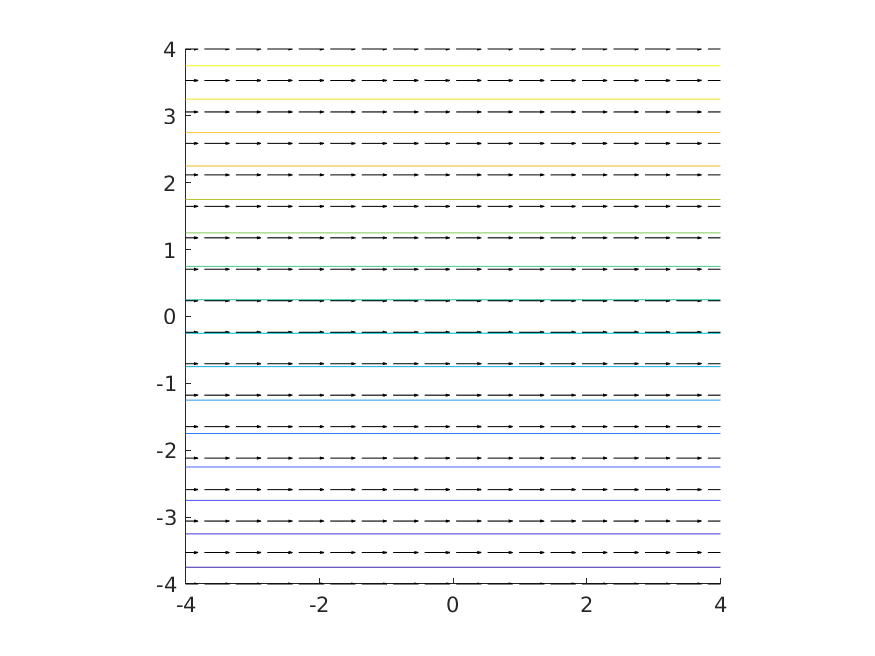
\includegraphics[width=35em]{mt_ex1_1}
    \centering
    \caption{Flow generated from $\Phi$}
    \label{fig:mt-1}
\end{figure}

Now let's see what happens when we apply Milne-Thomson, taking $a = 2$. Then we have
%
\begin{equation*}
    \Phi_{mt} = z + \frac{4}{z}
    ,
\end{equation*}
%
and hence
%
\begin{align*}
    \phi_{mt} &= x + \frac{4 x}{x^2 + y^2}, \\
    \psi_{mt} &= y - \frac{4 y}{x^2 + y^2}
    .
\end{align*}
%
The resulting flow is plotted below in Figure~\ref{fig:mt-2}. In this
figure, the streamline $\psi = 0$ is plotted below in black, and we can
see that it aligns perfectly with the circle $|z| = 2$. Note also that
velocity quivers at $|z| < 1$ where not plotted, due to their large
magnitude near the origin.
%
\begin{figure}[!ht]
    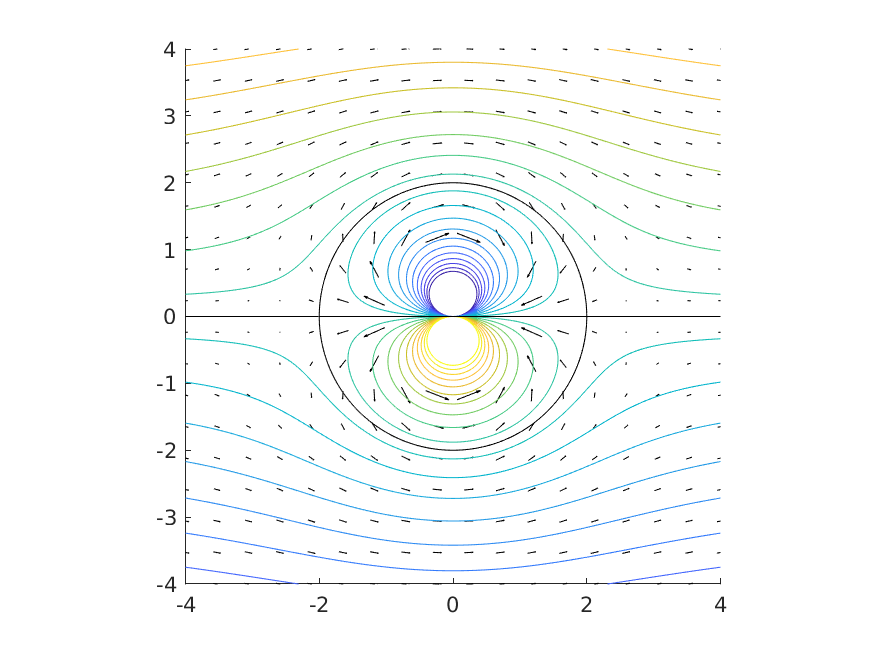
\includegraphics[width=35em]{mt_ex1_2}
    \centering
    \caption{Flow generated from $\Phi_{mt}$}
    \label{fig:mt-2}
\end{figure}

\textbf{Another example}


\end{document}
